\appendix
\addchap{Anhang}
\refstepcounter{chapter}

\section{Metriken aus dem Entwicklungsprozess}\label{appendix:metrics}

\begin{table}[H]
    \centering
    \begin{tabular}{p{6.5cm}p{8cm}} \toprule
    \textbf{\ac{CLOC}} & Anzahl der geänderten Zeilen im Quellcode. \\
    \multicolumn{2}{p{14.5cm}}{\textit{Wie viele Änderungen passieren in der Codebasis? \newline Wo finden die meisten Änderungen statt?}} \\ \midrule
    \textbf{\ac{CLOC} pro Entwickler} & Anzahl der geänderten Zeilen im Quellcode pro Entwickler. \\ 
    \multicolumn{2}{p{14.5cm}}{\textit{Wie viel Code ändert jeder im Team? \newline  Wer ist wie oft in welchem Modul?}} \\ \midrule
    \textbf{\ac{CLOC} pro Commit} & Anzahl der geänderten Zeilen im Quellcode pro Commit. \\ 
    \multicolumn{2}{p{14.5cm}}{\textit{Wie groß sind die Commits?}} \\ \midrule
    \textbf{Commits} & Gesamtzahl an Commits in einem bestimmten Zeitraum. \\ 
    \multicolumn{2}{p{14.5cm}}{\textit{Wie viel Änderungen wurden im Quellcode vorgenommen?}} \\ \midrule
    \textbf{Commits pro Entwickler} & Gesamtzahl an Commits in einem bestimmten Zeitraum pro Entwickler. \\ 
    \multicolumn{2}{p{14.5cm}}{\textit{Wie viel Änderungen wurden im Quellcode von einem Entwickler vorgenommen?}} \\ \midrule
    \textbf{Kommentare pro Commit} & Anzahl der Kommentare pro Commit. \\ 
    \multicolumn{2}{p{14.5cm}}{\textit{Wer arbeitet zusammen? \newline Wie viel wird zusammengearbeitet?}} \\ \midrule
    \textbf{Pull Requests} & Gesamtzahl an Pull Requests in einem bestimmten Zeitraum. \\ 
    \multicolumn{2}{p{14.5cm}}{\textit{Wird mit Pull Requests gearbeitet? \newline Werden Reviews gemacht?}} \\ \midrule
    \textbf{Gemergte Pull Requests} & Anzahl erfolgreicher Pull Requests in einem bestimmten Zeitraum. \\ 
    \multicolumn{2}{p{14.5cm}}{\textit{Wie oft werden erfolgreiche Änderungen in die Codebasis übernommen?}} \\ \midrule
    \textbf{Abgelehnte Pull Requests} & Anzahl abgelehnter Pull Requests in einem bestimmten Zeitraum. \\ 
    \multicolumn{2}{p{14.5cm}}{\textit{Wie oft werden Änderungen an der Codebasis abgelehnt? \newline Wie klar sind die Erwartungen des Teams an eine abgeschlossene Änderung (\ac{DoD})?}} \\ \midrule
    \textbf{Kommentare pro Pull Request} & Anzahl der Kommentare pro Pull Request. \\ 
    \multicolumn{2}{p{14.5cm}}{\textit{Wer arbeitet zusammen? \newline Wie viel wird zusammengearbeitet?}} \\ \bottomrule
    \end{tabular}
    \caption{Kennzahlen aus dem \ac{VCS}}\label{metrics-table-vcs}
  \end{table}
  
  \begin{table}[H]
    \centering
    \begin{tabular}{p{5cm}p{9.5cm}} \toprule
    \textbf{Burn Down} & Die Anzahl erledigte Arbeit über die Zeit. Liefert einen Richtwert, wo man sich gerade im Sprint befindet, verglichen zum Commitment. \\
    \multicolumn{2}{p{14.5cm}}{\textit{Erfüllt das Team seine Commitments? \newline Plant das Team seine Arbeit realistisch?}} \\ \midrule
    \textbf{Velocity} & Eine relative Messung der Konsistenz erledigter Arbeit über die Sprints. \\
    \multicolumn{2}{p{14.5cm}}{\textit{Wie konsistent arbeitet das Team?}} \\ \midrule
    \textbf{Cumulative Flow} & Zeigt wie viel Aufgaben nach Status dem Team zugewiesen sind über die Zeit. \\
    \multicolumn{2}{p{14.5cm}}{\textit{Gibt es Engpässe oder Schwachstellen im Prozess? \newline Müssen gewisse Abläufe im Prozess optimiert werden?}} \\ \midrule
    \textbf{Lead Time} & Zeit zwischen Start und Abschluss einer Aufgabe, vor allem interessant bei Kanban. \\
    \multicolumn{2}{p{14.5cm}}{\textit{Wie schnell können Aufgaben vom Team erledigt werden? \newline Wie lange dauert die Umsetzung eines neuen Features?}} \\ \midrule
    \textbf{Bug Counts} & Die Anzahl an Bugs über die Zeit. \\
    \multicolumn{2}{p{14.5cm}}{\textit{Wie viele Fehler werden vom Team im Entwicklungsprozess übersehen? \newline Wie viel ungeplante Arbeit kam zum Sprint dazu?}} \\ \midrule
    \textbf{Bug-Erzeugungsrate} & Anzahl Bugs nach Erstellungsdatum. \\
    \multicolumn{2}{p{14.5cm}}{\textit{Wie viele Fehler wurden zu einem bestimmten Zeitpunkt erzeugt?}} \\ \midrule
    \textbf{Bug-Fertigstellungsrate} & Anzahl Bugs nach Erledigungsdatum. \\
    \multicolumn{2}{p{14.5cm}}{\textit{Wie viele Fehler wurden zu einem bestimmten Zeitpunkt beseitgt?}} \\ \midrule
    \textbf{Aufgaben-Volumen} & Ist die Anzahl der Aufgaben und kann der Schätzung gegenübergestellt werden, um die Größe der Aufgaben oder ungeplante Arbeit aufzuzeigen. \\
    \multicolumn{2}{p{14.5cm}}{\textit{Wie viel ungeplante Arbeit kam zum Sprint dazu? \newline Wie groß ist die durchschnittliche Aufgabe? Gibt es Ausreißer?}} \\ \midrule
    \textbf{Aufgaben-Rückfälligkeit} & Zeigt auf, wie oft Aufgaben im Arbeitsablauf rückwärts gehen. \\
    \multicolumn{2}{p{14.5cm}}{\textit{Wie viele Aufgaben werden wieder in einen vorhergehenden Status gesetzt? \newline Gibt es Probleme beim Verständnis der Aufgaben? \newline Wie klar sind die Erwartungen des Teams an eine abgeschlossene Änderung (DoD)?}} \\ \bottomrule
    \end{tabular}
    \caption{Kennzahlen aus dem \ac{PTS}}\label{metrics-table-pts}
  \end{table}
  
  \begin{table}[H]
    \centering
    \begin{tabular}{p{6.5cm}p{8cm}} \toprule
    \textbf{Build-Dauer} & Geschätzte und tatsächliche Dauer der Builds. \\
    \multicolumn{2}{p{14.5cm}}{\textit{Wie lange dauert es ein Softwareartefakt zu erstellen? \newline Wie verändert sich die Dauer der Erstellung eines Softwareartefakts über die Zeit?}} \\ \midrule
    \textbf{Build-Status} & Es können die Anzahl der erfolgreichen und fehlerhaften Builds gegenüber gestellt werden. \\
    \multicolumn{2}{p{14.5cm}}{\textit{Gibt es ein Problem im Freigabeprozess?}} \\ \midrule
    \textbf{Build-Frequenz} & Wie oft wird ein Build ausgelöst. \\
    \multicolumn{2}{p{14.5cm}}{\textit{Wird oft genug ein neues Softwareartefakt erstellt?}} \\ \midrule
    \textbf{Test Reports} & Anzahl erfolgreicher und fehlerhafter Tests, Gesamtdauer der Tests. \\
    \multicolumn{2}{p{14.5cm}}{\textit{Wie lange dauert ein kompletter Testdurchlauf? \newline Gibt es Tests, die optimiert werden müssen? \newline Wie oft werden fehlerhafte Tests in die Codebasis aufgenommen?}} \\ \midrule
    \textbf{Code Coverage} & Wie viel Prozent des Quellcodes ist mit Tests abgedeckt. \\
    \multicolumn{2}{p{14.5cm}}{\textit{Gibt es Module, die nicht oder schlecht getestet sind? \newline Wie sieht die Entwicklung der Testabdeckung über die Zeit aus?}} \\ \midrule
    \textbf{Stresstests oder Benchmarking} & Hier kann das Ergebnisse die unterschiedliche Reports sein. \\
    \multicolumn{2}{p{14.5cm}}{\textit{Ist das Produkt auch noch unter Last verwendbar? \newline Wie verändert sich die Leistung über die Zeit?}} \\ \bottomrule
    \end{tabular}
    \caption{Kennzahlen aus den \ac{CI}- und \ac{CD}}-Systemen\label{metrics-table-cicd}
  \end{table}
  
  \begin{table}[H]
    \centering
    \begin{tabular}{p{5cm}p{9.5cm}} \toprule
    \textbf{CPU Nutzung} & Auslastung der Prozessoren über die Zeit. \\
    \textbf{Heap Size} & Auslastung des Heap über die Zeit. \\
    \multicolumn{2}{p{14.5cm}}{\textit{Arbeitet die Software technisch effizient? \newline Ist die Hardware ausreichend? \newline Gibt es eine erhöhte Auslastung nach einer Änderung?}} \\ \midrule
    \textbf{Fehlerraten} & Anzahl Fehler über die Zeit (kann aus dem Logging kommen). \\
    \multicolumn{2}{p{14.5cm}}{\textit{Werden seit einer Änderung mehr Fehler produziert? \newline Wie entwickelt sich die Fehlerrate über die Zeit?}} \\ \midrule
    \textbf{Antwortzeiten} & Dauer der Verarbeitung bestimmter Anfragen. \\
    \multicolumn{2}{p{14.5cm}}{\textit{Reagiert und arbeitet das Produkt noch schnell genug? \newline Gibt es Geschwindigkeitsprobleme seit der letzen Änderung? \newline Wie entwickeln sich die Antwortzeiten über die Zeit?}} \\ \midrule
    \textbf{Benutzeranzahl} & Anzahl gleichzeitiger Benutzer in der Applikation über die Zeit. \\
    \multicolumn{2}{p{14.5cm}}{\textit{Wie entwickeln sich die Benutzerzahlen mit der Zeit? \newline Geht das Produkt in die richtige Richtung? \newline Ist mit höheren Lasten zu rechnen?}} \\ \midrule
    \textbf{Aufenthaltsdauer} & Verweildauer der Benutzer auf bestimmten Seiten. \\
    \multicolumn{2}{p{14.5cm}}{\textit{Welche Features werden besonders oft / selten genutzt? \newline Hat das neue Feature den gewünschten Effekt? Wird es genutzt?}} \\ \midrule
    \textbf{Conversion Rate} & Anzahl Benutzer die zu Kunden wurden. \\
    \multicolumn{2}{p{14.5cm}}{\textit{Wie entwicklt sich die Zahl der zahlenden Neukunden?}} \\ \midrule
    \textbf{Semantisches Logging} & Strukturierte Daten aus dem Logging. \\
    \multicolumn{2}{p{14.5cm}}{\textit{Hier können Daten zu anderen Fragen gesammelt werden, die für den Prozess wichtig sind.}} \\ \bottomrule
    \textbf{Verfügbarkeit} & Verfügbarkeit der Applikation über die Zeit. \\
    \multicolumn{2}{p{14.5cm}}{\textit{Wie hoch ist die Ausfallsicherheit? \newline Wie lange war die Applikation nicht verfügbar?}} \\ \bottomrule
    \end{tabular}
    \caption{Kennzahlen aus den \ac{APM}- und \ac{BI}}-Systemen\label{metrics-table-apm}
  \end{table}

\newpage
\section{Ergebnisse Analyse Retrospektiven}\label{appendix:retros}

\subsection*{Welche guten Entscheidungen haben wir getroffen?}
\begin{enumerate}
    \item sprint (4)
    \item einblick (3)
    \item onboarding (3)
    \item pair (3)
    \item programming (3)
    \item system (3)
    \item arbeit (2)
    \item daily (2)
    \item erledig (2)
    \item information (2)
    \item issu (2)
    \item po (2)
    \item review (2)
    \item reviewing (2)
    \item schnell (2)
    \item stori (2)
    \item urlaub (2)
    \item angenehm (1)
    \item annehm (1)
    \item cloud (1)
    \item dailys (1)
    \item diskussion (1)
    \item dor (1)
    \item durchgefuhrt (1)
    \item einfach (1)
\end{enumerate}

\subsection*{Was haben wir gelernt?}
\begin{enumerate}
    \item sprint (7)
    \item onboarding (4)
    \item team (4)
    \item arbeit (3)
    \item besprech (3)
    \item board (3)
    \item datenfluss (3)
    \item issus (3)
    \item planungswoch (3)
    \item retro (3)
    \item richtlini (3)
    \item system (3)
    \item uberblick (3)
    \item umgestellt (3)
    \item altlast (2)
    \item analogboard (2)
    \item approved (2)
    \item backlog (2)
    \item daily (2)
    \item digital (2)
    \item direkt (2)
    \item genau (2)
    \item impediment (2)
    \item infrastruktur (2)
    \item iso (2)
\end{enumerate}

\subsection*{Was können wir besser machen?}
\begin{enumerate}
    \item sprint (10)
    \item review (7)
    \item checklist (4)
    \item daily (4)
    \item display (4)
    \item doku (4)
    \item issu (4)
    \item po (4)
    \item einarbeitung (3)
    \item einkalkuli (3)
    \item gross (3)
    \item https (3)
    \item java (3)
    \item stori (3)
    \item ablauf (2)
    \item anderung (2)
    \item arbeitspaket (2)
    \item aufnehm (2)
    \item aufteil (2)
    \item backlog (2)
    \item blocked (2)
    \item dokumenti (2)
    \item erledig (2)
    \item geplant (2)
    \item geschatzt (2)
\end{enumerate}

\subsection*{Was nervt uns noch immer?}
\begin{enumerate}
    \item problem (11)
    \item updat (11)
    \item apis (10)
    \item archiv (10)
    \item erreichbar (10)
    \item infrastruktur (10)
    \item jenkin (10)
    \item test (9)
    \item umgebung (9)
    \item dba (8)
    \item eingerichtet (8)
    \item jndi (8)
    \item laut (8)
    \item verwendbar (8)
    \item arbeit (7)
    \item impediment (7)
    \item iso (7)
    \item lang (7)
    \item mitarbeit (6)
    \item mehr (5)
    \item wichtig (5)
    \item anderung (4)
    \item aufteilbar (4)
    \item gross (4)
    \item klar (4)
\end{enumerate}

\newpage
\section{Umfrage Scrum Team}

\subsection{Fragebogen}\label{appendix:questions}
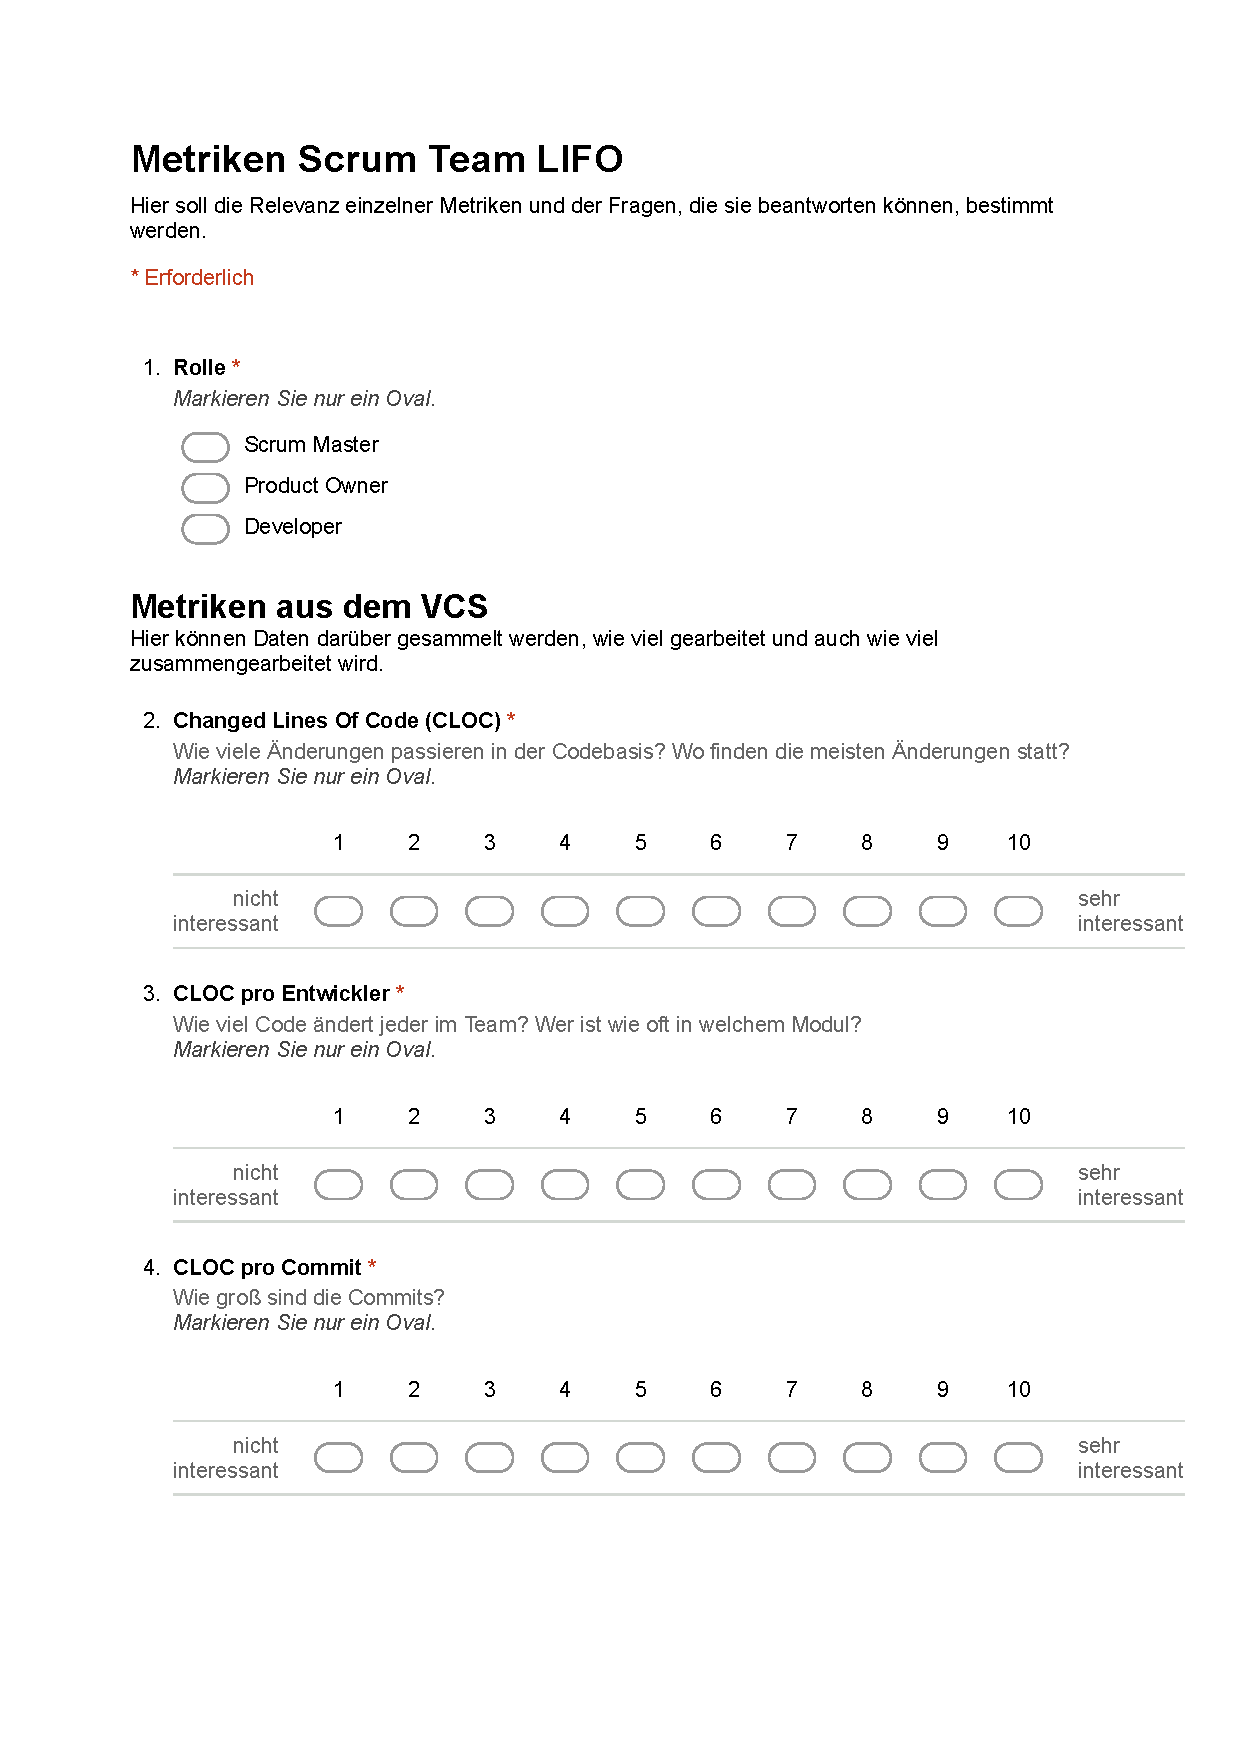
\includepdf[pages=-, scale=0.9, pagecommand={\thispagestyle{plain}}]{appendix/fragebogen.pdf}

\subsection{Ergebnisse}\label{appendix:answers}
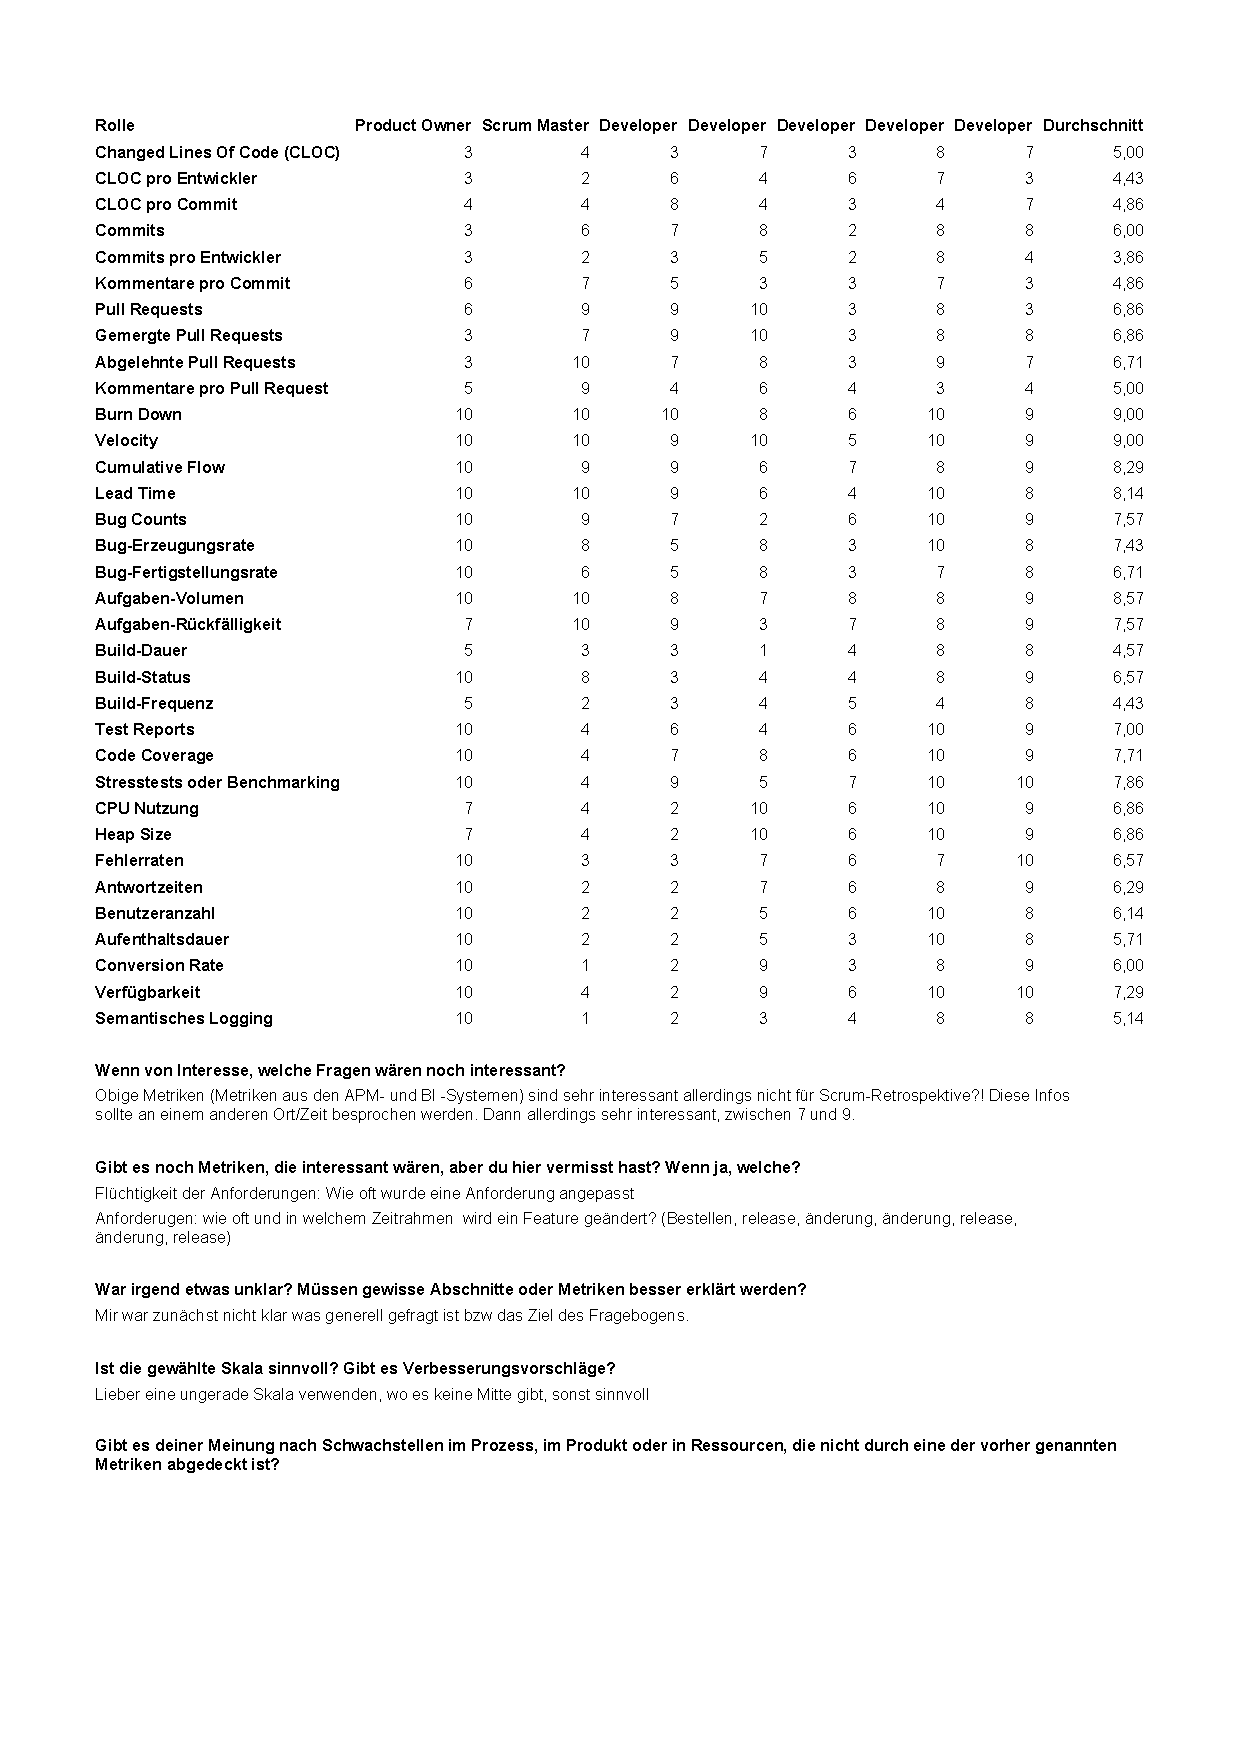
\includepdf[pages=-, scale=0.9, pagecommand={\thispagestyle{plain}}]{appendix/fragebogen-ergebnis.pdf}
